\section{Across-Environment Generalization}
\label{appendix:cont_to_bern_headless}

We evaluated Headless-AD's ability to generalize skills learned in one domain to another.
We trained Headless-AD on Contextual Bandits and subsequently assessed its performance on Bernoulli Bandits. To align with the Contextual Bandit setting, we introduced a random vector to serve as the state in the Bernoulli Bandit environment, effectively transforming it into a single-context Contextual Bandit scenario with Bernoulli-distributed rewards.

\Cref{fig:cont_to_bern_headless} presents the results of these cross-domain experiments. Headless-AD not only adapted to the new domain but also maintained a satisfactory performance level, highlighting the model's capacity for cross-environment application.

\begin{figure*}[h]
    \vskip 0.2in
    \centering
    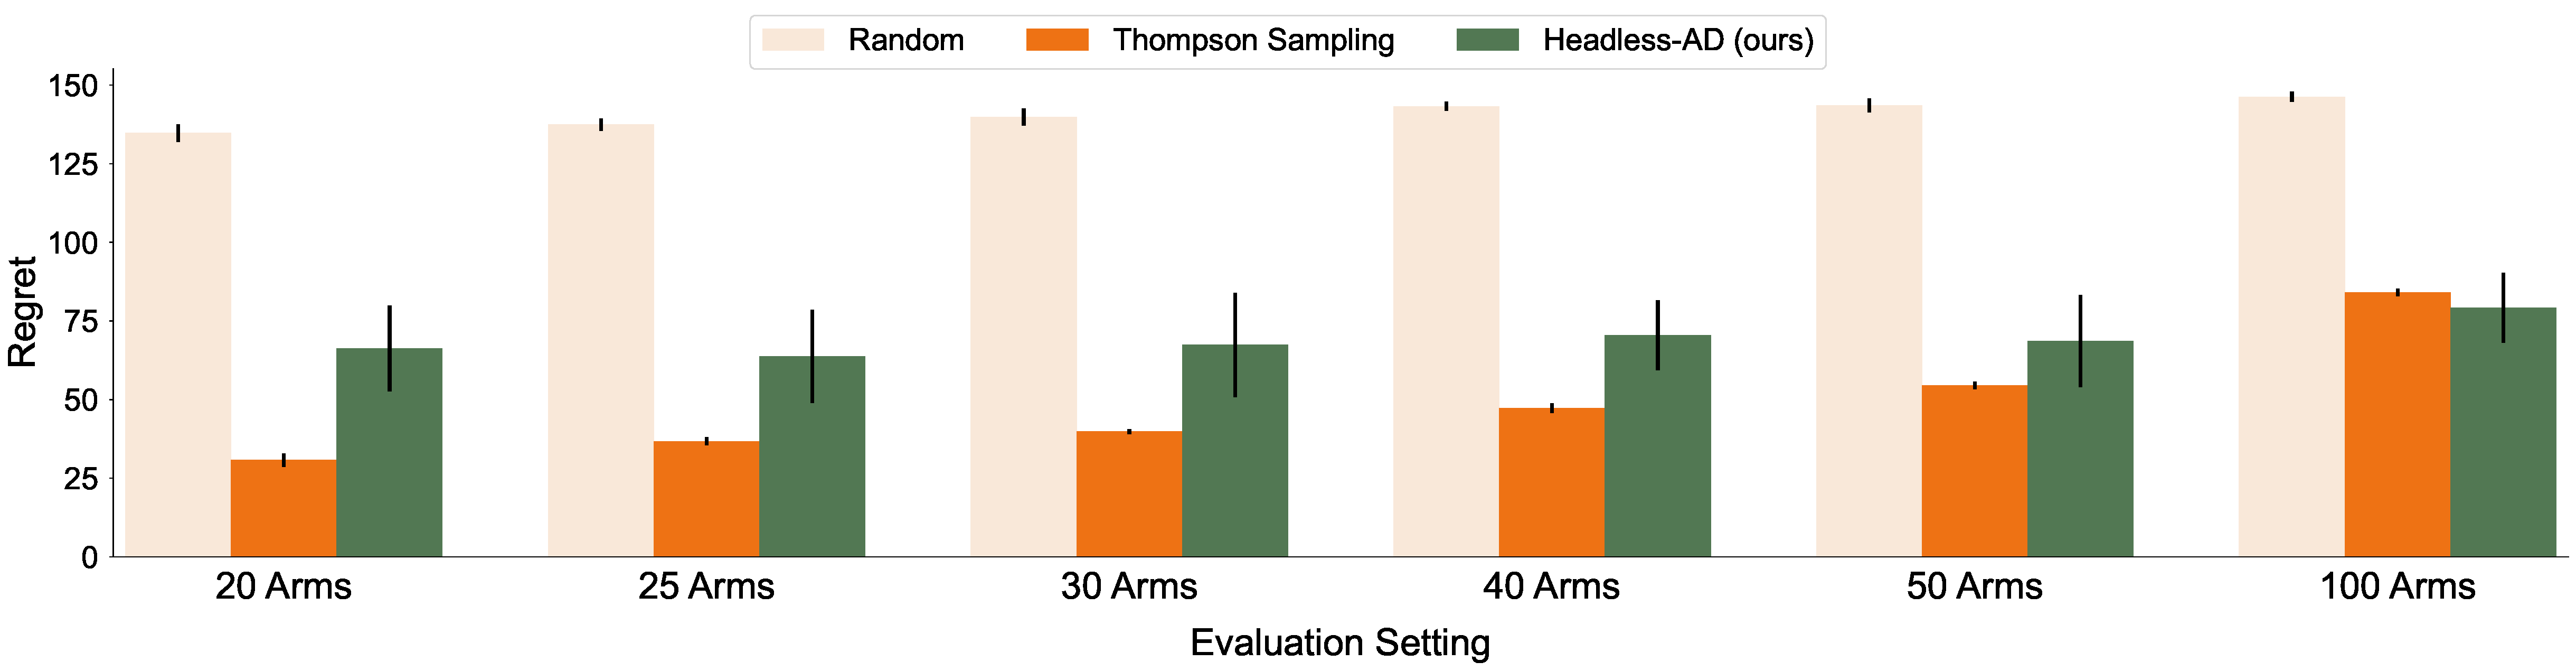
\includegraphics[width=0.7\textwidth]{images/cont_to_bern_headless_25.pdf}
    \caption{\textbf{Evaluation of Across-Environment Generalization:} This graph illustrates the performance of the Headless-AD model, which was initially trained on a Contextual Bandit setting and then evaluated on a Bernoulli Bandit environment. The experiment aimed to assess the model's generalization capabilities across novel environments. As shown, Headless-AD achieves a decent performance across various configurations with different numbers of arms, demonstrating its potential for across-environment usage.}
    \label{fig:cont_to_bern_headless}
    \vskip -0.2in
\end{figure*}
